\documentclass[a4paper, 12pt]{article}
\usepackage{graphicx}
\usepackage[margin=2cm]{geometry}
\usepackage[hidelinks]{hyperref}
\usepackage[croatian]{babel}
\usepackage[sorting=none]{biblatex}
    \addbibresource{ref.bib}
\usepackage{float}


% Boje za kod:
\usepackage{xcolor,graphicx}
\usepackage{listings}

\definecolor{solarized-base03}{RGB}{0, 43, 54}
\definecolor{solarized-base02}{RGB}{7, 54, 66}
\definecolor{solarized-base01}{RGB}{88, 110, 117}
\definecolor{solarized-base00}{RGB}{101, 123, 131}
\definecolor{solarized-base0}{RGB}{131, 148, 150}
\definecolor{solarized-base1}{RGB}{147, 161, 161}
\definecolor{solarized-base2}{RGB}{238, 232, 213}
\definecolor{solarized-base3}{RGB}{253, 246, 227}
\definecolor{solarized-yellow}{RGB}{181, 137, 0}
\definecolor{solarized-orange}{RGB}{203, 75, 22}
\definecolor{solarized-red}{RGB}{220, 50, 47}
\definecolor{solarized-magenta}{RGB}{211, 54, 130}
\definecolor{solarized-violet}{RGB}{108, 113, 196}
\definecolor{solarized-blue}{RGB}{38, 139, 210}
\definecolor{solarized-cyan}{RGB}{42, 161, 198}
\definecolor{solarized-green}{RGB}{133, 153, 0}

\lstset{
  basicstyle=\footnotesize\ttfamily\color{solarized-base00},
  keywordstyle=\color{solarized-blue}\bfseries,
  commentstyle=\color{solarized-base1},
  stringstyle=\color{solarized-cyan},
  identifierstyle=\color{solarized-violet},
  numberstyle=\tiny\color{solarized-base01},
  numbers=left,
  firstnumber=1,
  stepnumber=1,
  showstringspaces=false,
  tabsize=4,
  frame=none,
  framerule=1pt,
  framexleftmargin=5pt,
  framexrightmargin=5pt,
  framextopmargin=3pt,
  framexbottommargin=3pt,
  backgroundcolor=\color{solarized-base3},
  rulecolor=\color{solarized-base01},
  breaklines=true,
  breakatwhitespace=true,
  language=C++
}


\begin{document}
\noindent
Univerzitet u Sarajevu\\
Elektrotehnički fakultet\\
Predmet: Uvod u digitalnu obradu slike\\
Predmetni profesor: prof. dr Emir Sokić\\
Autor: Berina Biberović\\
Akademska godina: 2022/2023.


\begin{center}
    \section*{Tutorijal 6}
    \subsection*{Template matching}
\end{center}

\textit{Template matching} ili podudaranje predložaka je metoda za tražnje i nalaženje slike predloška u većoj slici. OpenCV ima funkciju \lstinline{cv::matchTemplate()} koja radi upravo to. Ta funkcija stavlja sliku predloška preko ulazne velike slike (kao 2D konvolucija) i upoređuje predložak i djelić ulazne slike ispod predloška. Kako predložak treba biti pravougaonik, može biti da nije cijeli pravougaonik relevantan za traženje onoga što nam treba iz velike ulazne slike - u tom slučaju može se koristiti maska da se izoluje dio predloška koji se treba koristiti da se nađe podudaranje. Detaljnije ćemo kasnije pričati o ovome.

Sljedeći primjer ilustruje kako uz pomoć šablona (tj. predloška) možemo naći da li se na ulaznoj slici nalazi traženi šablon.

\begin{lstlisting}
#include <opencv4/opencv2/imgcodecs.hpp>
#include <opencv4/opencv2/highgui.hpp>
#include <opencv4/opencv2/imgproc.hpp>
#include <opencv4/opencv2/core.hpp>

int main() {

    // Ucitavanje ulazne slike:
    cv::Mat slika = cv::imread("../Moje karte/IMG_0002.JPG", cv::IMREAD_COLOR);
    // Ucitavanje predloska:
    cv::Mat temp = cv::imread("../Moje karte predlosci/herc.JPG", cv::IMREAD_COLOR);

    cv::Mat rezultat;

    // Ove varijable su nam potrebne za funkciju za template matching:
    int rezcol, rezrow;
    rezcol = slika.cols - temp.cols + 1;
    rezrow = slika.rows - temp.rows + 1;

    rezultat.create(rezrow, rezcol, CV_32FC1);

    cv::matchTemplate(slika, temp, rezultat, cv::TM_CCORR_NORMED);

    // Sad racunamo koliko se podudaraju i gdje:
    double min_vr, max_vr;
    cv::Point min_lok, max_lok, match_lok;

    cv::minMaxLoc(rezultat, &min_vr, &max_vr, &min_lok, &max_lok);
    match_lok = max_lok;

    // Sad trebamo nacrtati gdje je template nadjen:
    cv::rectangle(slika, match_lok, cv::Point(match_lok.x + temp.cols, match_lok.y + temp.rows), cv::Scalar(0, 0, 255), 2, 8, 0);

    cv::imshow("Rezultat template matchinga", slika);
    cv::waitKey();

    return 0;
}
\end{lstlisting}

U prethodnom primjeru su korištene igraće karte kako bi se demonstriralo kako radi \textit{template matching} u OpenCV-u. Ulazna slika je prikazana na slici \ref{sl1}, a šablon je prikazan na slici \ref{sl2}.

\begin{figure}[H]
    \centering
    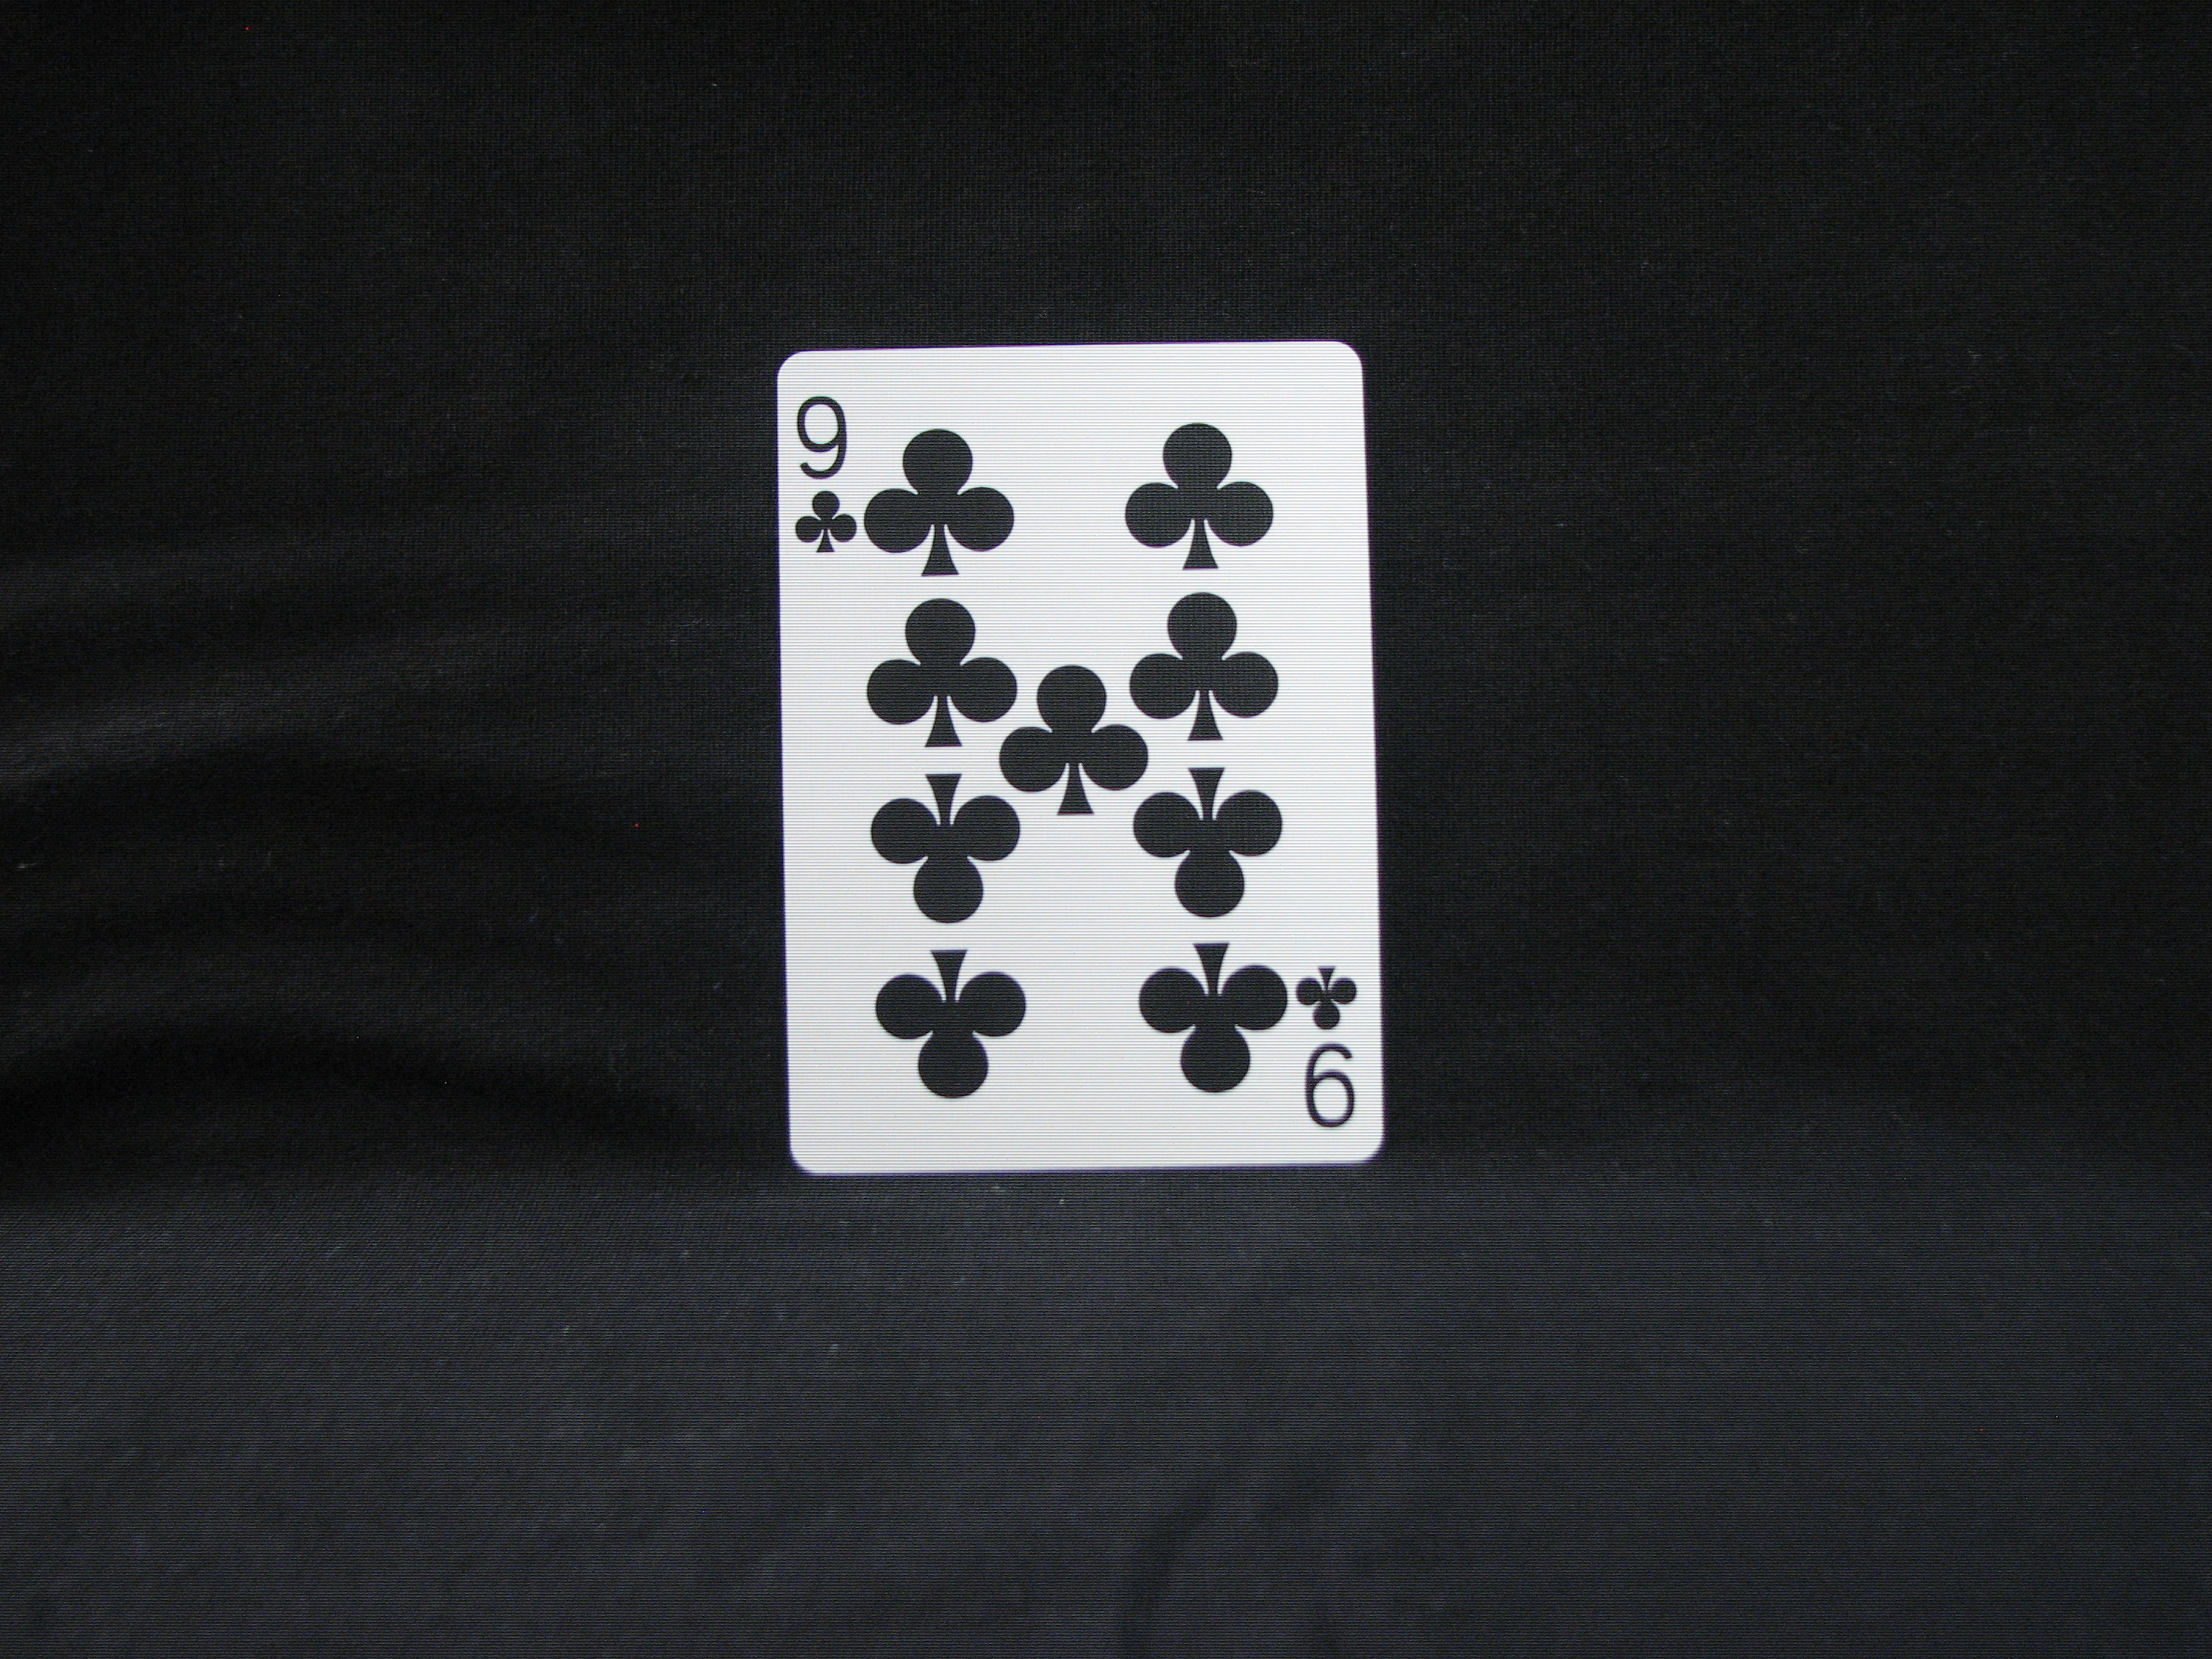
\includegraphics[width=\textwidth]{Slike/IMG_0007.jpg}
    \caption{Ulazna slika za prvi primjer}
    \label{sl1}
\end{figure}

\begin{figure}[H]
    \centering
    
\includegraphics{Slike/tref.jpg}
    \caption{Predložak za prvi primjer}
    \label{sl2}
\end{figure}

Prvo učitamo ulaznu sliku i predložak, na osnovu njihovih veličina računamo varijable \lstinline{rezcol} i \lstinline{rezrow}. Te dvije varijable koristimo kako bismo napravili novu instancu klase \lstinline{cv::Mat} u koju ćemo smještati rezultat \textit{template matching}-a. To radimo preko instance funkcije \lstinline{cv::Mat::create} koja alocira mjesto za novu sliku preko broja redova, kolona i tipa kojoj joj proslijedimo. Kada smo sve to uradili, možemo pozvati funkciju \lstinline{cv::matchTemplate} koja redom prima: ulaznu sliku, šablon, sliku u koju smještamo rezultat \textit{template matching}-a i parametar koji specificira metodu poređenja (postoji i peti parametar koji je predefiniran ukoliko ga mi ne proslijedimo, a to je upravo maska o kojoj smo ramnije pričali).

Nakon što smo dobili rezultat, koristimo funkciju \lstinline{cv::minMaxLoc} koja nalazi najmanji i najveći element u nizu (u ovom slučaju instanca tipa \lstinline{cv::Mat} i njihove lokacije. Trebamo ovdje naglasiti da ova funkcija ne radi sa multi-kanalnim nizovima (potrebno je iskorisiti funkciju \lstinline{cv::Mat::reshape} onda). Kada smo našli minimalni i maksimalni element i njihovu lokaciju (u ovom kontekstu to znači gdje se najmanje i najviše šablon podudara sa ulaznom slikom), onda je potrebno da na lokaciji maksimalnog elementa nacrtamo pravougaonik koji odgovara šablonu na ulaznoj slici.

Koristimo funkciju \lstinline{cv::rectangle} za to - ta funkcija prima niz na kojem trebamo nacrtati pravougaonik, lokaciju gdje trebamo nacrtati pravougaonik (lijeva gornja ivica pravougaonika), desna donja ivica pravougaonika, boju kojom želimo da nacrtamo pravougaonik (u primjeru je to crvena boja), debljina linije, tip linije i broj tzv. frakcionih bitova u koordinatama tačaka navedenih ivica. Rezultat je prikazan na slici \ref{sl3} gdje vidimo da je uspješno nađen traženi šablon.

\begin{figure}
    \centering
    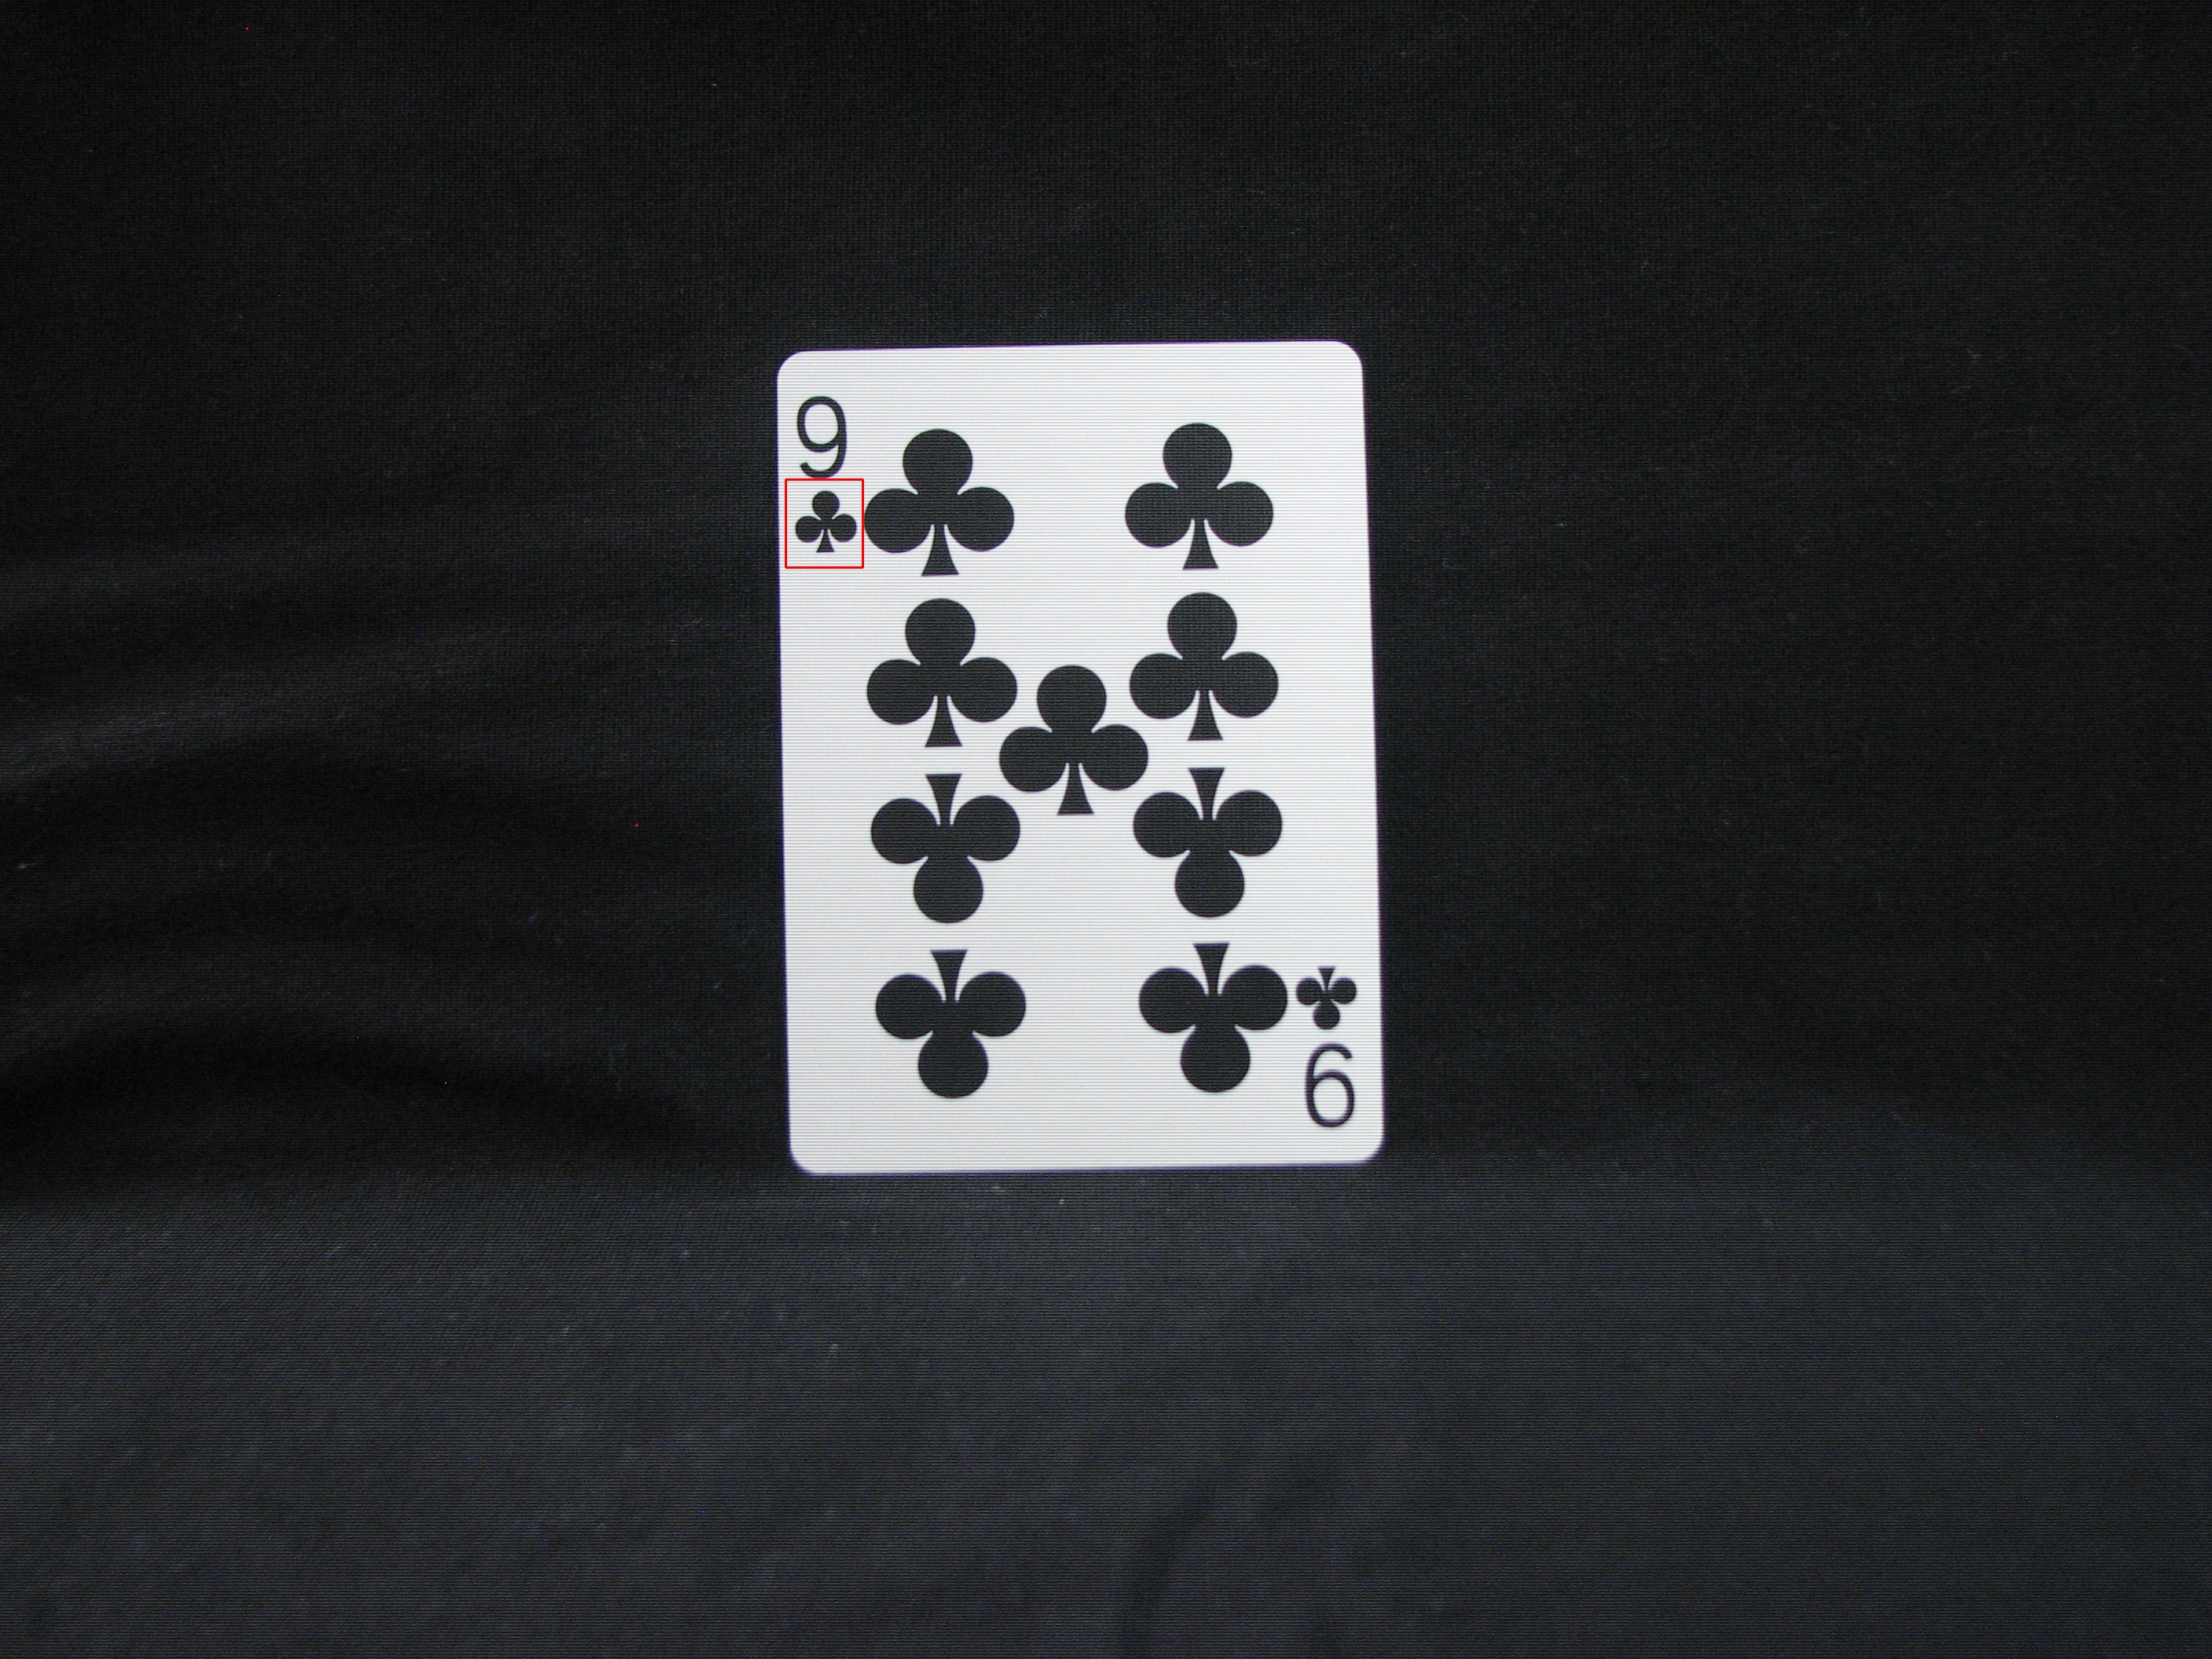
\includegraphics[width=\textwidth]{Slike/rezultat.jpg}
    \caption{Rezultat \textit{template matching}-a u prvom primjeru}
    \label{sl3}
\end{figure}

Prethodno pokazani primjer nam pokazuje da je korištenje \textit{template matching}-a veoma neprecizna metoda za pronalaženje predmeta/lika na ulaznoj slici. Zapravo je pokazan najjednostavniji primjer - predložak je bio uzet sa ulazne slike, tako da je logično da će se naći odgovarajuće podudaranje. Problem nastaje ukoliko imamo više različitih karata istog znaka koji su udaljeni različito od kamere ili ako su karte rotirane za neki ugao. U tom slučaju dolazimo do problema jer \textit{template matching} samo provlači šablon iznad ulazne slike i gleda podudaranje - ali ako imamo zarotirani simbol, šta onda uraditi?

U nastavku će biti navedene funkcije koje su korisne upravo za prethodni slučaj:

\begin{itemize}
    \item \lstinline{cv::resize} funkcija kojom možemo smanjiti ili povećati predložak ukoliko je to potrebno.
    \begin{lstlisting}
        void cv::resize(InputArray ulaz, OutputArray izlaz, Size dsize, double fx = 0, double fy = 0, int interpolacija = cv::INTER_LINEAR)
    \end{lstlisting}
    Parametar \lstinline{ulaz} predstavlja sliku čiju veličinu želimo promijeniti, \lstinline{izlaz} je rezultantna slika nakon mijenjanja veličine, \lstinline{dsize} je veličina izlazne slike, \lstinline{fx} je faktor skaliranja po horizontalnoj osi, \lstinline{fy} je faktor skaliranja po vertikalnoj osi, a \lstinline{interpolacija} predstavlja način (metodu) interpolacije.
    \item \lstinline{cv::getRotationMatrix2D} funkcija računa afinu matricu 2D rotacije (izvršena je neka linearna transformacija i/ili translacija). 
    \begin{lstlisting}
        cv::Mat cv::getRotationMatrix2D(Point2f centar, double ugao, double skala)
    \end{lstlisting}
    Parametar \lstinline{centar} predstavlja centar rotacije izvorne slike, \lstinline{ugao} predstavlja ugao za koji rotiramo sliku (može biti pozitivan, u smjeru kretanja kazaljke na satu, ili negativan, suprotno od smjera kretanja kazaljke na satu) i \lstinline{skala} predstavlja faktor izotropnog skaliranja (skaliranje invarijantno na bilo koji pravac).
    \item \lstinline{cv::warpAffine} funkcija koja radi afinu transformaciju sliku.
    \begin{lstlisting}
        void cv::warpAffine(InputArray ulaz, OutputArray izlaz, InputArray M, Size dsize, int flag = cv::INTER_LINEAR, int modus_granice = cv::BORDER_CONSTANT, const Scalar & vrijednost_granice = cv::Scalar())
    \end{lstlisting}
    Parametar \lstinline{ulaz} je ulazna slika koja se rotira, \lstinline{izlaz} je rezultat nakon rotiranja, \lstinline{M} je transformacijska matrica, \lstinline{dsize} je veličina izlazne slike, \lstinline{flag} kombinacija interpolacijskih metoda i opcionalnog \textit{flag}-a \lstinline{cv::WARP_INVERSE_MAP} koja znači da je \lstinline{M} inverzna transformacija, \lstinline{modus_granice} predstavlja metodu ekstrapolacije piksela i \lstinline{vrijednost_granice} predstavlja vrijednost koja se koristi ukoliko je granica konstantna (postavljena je inače na 0).
\end{itemize}

Primijetit ćete da je implementacija ovih funkcija na realističnim slučajevima nepraktična. Postavlja se pitanje - za šta uopšte služi \textit{template matching}? U realnosti se mogu koristiti za npr. testiranje kvaliteta u proizvodnji ili navigaciju mobilnih robota. U suštini, \textit{template matching} je koristan za predloške koji nemaju tzv. jake osobine ili kada je većina predloška dio ulazne slike. Primijetit ćete prilikom rada na laboratorijskoj vježbi da je \textit{template matching} spor, upravo zbog toga što se prelazi preko cijele ulazne slike sa predloškom - to mnogo usporava proces (šta ako imamo mnogo slika ili ako su slike velike?). 

\subsection*{Napomene}

Korištena tema za prikaz C++ koda na tutorijalima je \href{https://ethanschoonover.com/solarized/}{\lstinline{solarized}}\cite{solarized}.

\printbibliography


\end{document}
